\hypertarget{algorytm_8cpp}{\section{\-Dokumentacja pliku algorytm.\-cpp}
\label{algorytm_8cpp}\index{algorytm.\-cpp@{algorytm.\-cpp}}
}


plik zawiera definicje metod klas zdefiniowanych w pliku \hyperlink{algorytm_8hh}{algorytm.\-hh}  


{\ttfamily \#include \char`\"{}algorytm.\-hh\char`\"{}}\*
\-Wykres zależności załączania dla algorytm.\-cpp\-:
\nopagebreak
\begin{figure}[H]
\begin{center}
\leavevmode
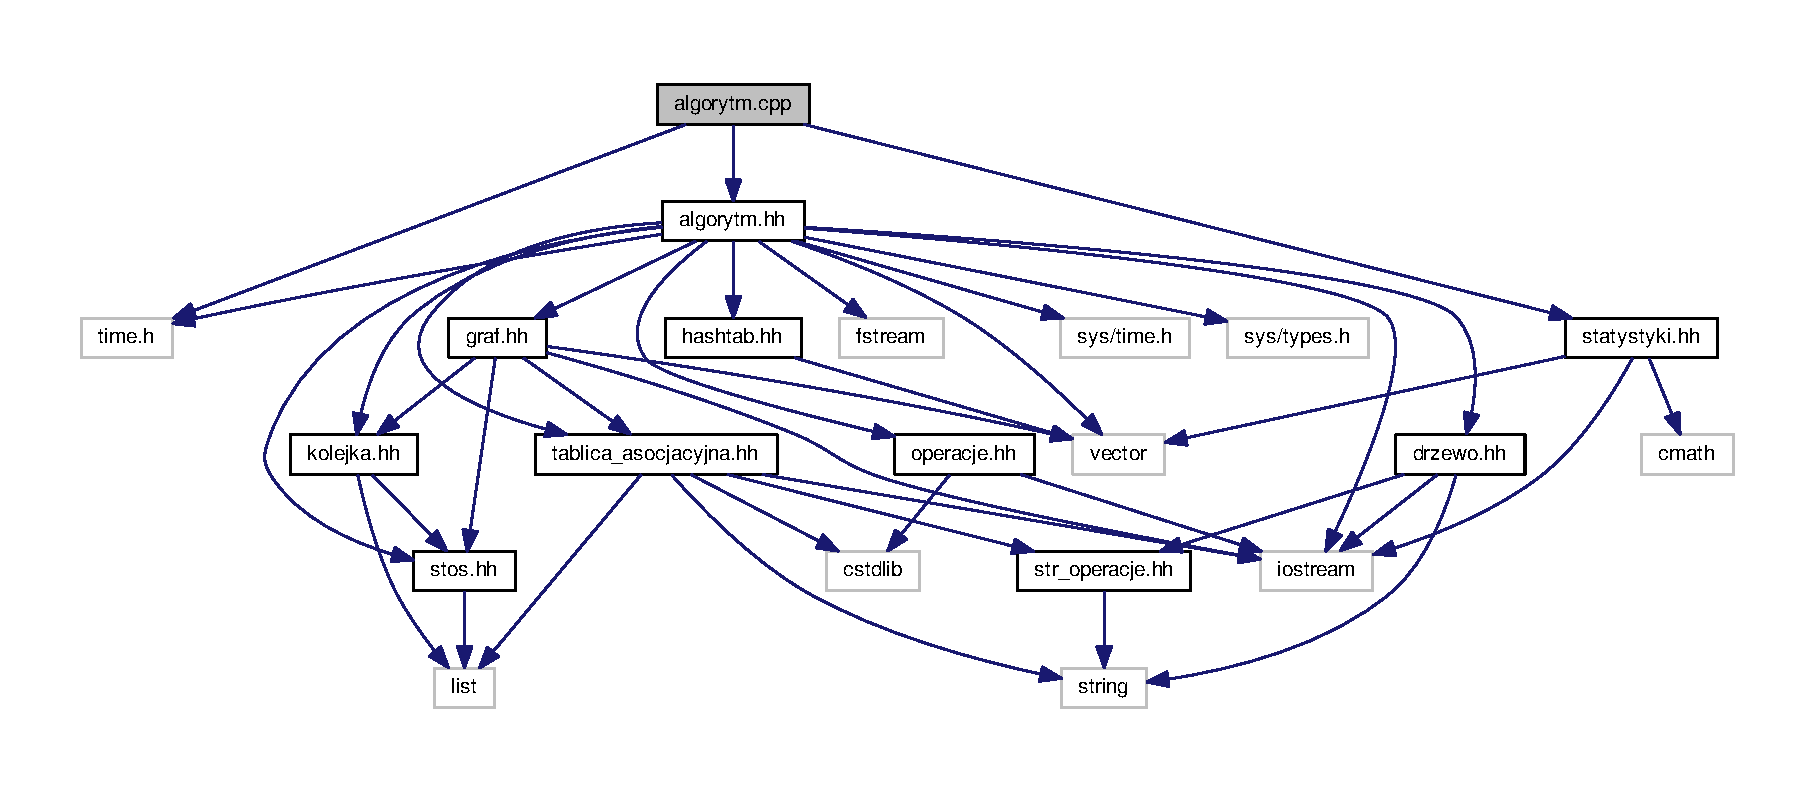
\includegraphics[width=350pt]{algorytm_8cpp__incl}
\end{center}
\end{figure}


\subsection{\-Opis szczegółowy}
plik zawiera definicje metod klas zdefiniowanych w pliku \hyperlink{algorytm_8hh}{algorytm.\-hh} 

\-Definicja w pliku \hyperlink{algorytm_8cpp_source}{algorytm.\-cpp}.

